\documentclass[a4paper,11pt]{article}
\usepackage{float}
\usepackage{amsmath}
\usepackage{amssymb}
\usepackage{fullpage}
\usepackage{rotating}
\usepackage{tikz} \usetikzlibrary{trees}
\usepackage{pbox}
\usepackage{algorithm}
\usepackage[noend]{algpseudocode}
\usepackage{listings}
\usepackage{hyperref}
\usepackage{courier}



\usepackage{siunitx}
\sisetup{per=slash, load=abbr}

\usepackage{tikz}
% \usetikzlibrary{calc,angles,positioning,intersections}
\usepackage{pgfplots}
\pgfplotsset{width=7cm, height=10cm, compat=1.4, every axis/.append style={thick}}



\newcommand{\AnyCond}[1]{\text{Any}(#1)}
\newcommand{\BoundedCond}[1]{\text{Bounded}(#1)}
\newcommand{\Constraint}[1]{\textsc{#1}}
\newcommand{\DepProps}{\textit{DepProps}}
\newcommand{\Distinct}{\Constraint{Distinct}}
\newcommand{\Failed}{\text{Failed}}
\newcommand{\FailedCond}[1]{\text{Failed}(#1)}
\newcommand{\FixedCond}[1]{\text{Fixed}(#1)}
\newcommand{\Fixpoint}{\text{AtFixpt}}
\newcommand{\NoneCond}[1]{\text{None}(#1)}
\newcommand{\Gecode}{\textit{Gecode}}
\newcommand{\GIST}{\textit{GIST}}
\newcommand{\Propagate}{\text{Propagate}}
\newcommand{\PropConds}[1]{\text{PropConds}(#1)}
\newcommand{\Sequence}[1]{\left[#1\right]}
\newcommand{\Set}[1]{\left\{#1\right\}}
\newcommand{\Subsumed}{\text{Subsumed}}
\newcommand{\Tuple}[1]{\left\langle#1\right\rangle}
\newcommand{\Unknown}{\text{Unknown}}

\pagestyle{empty}

\renewcommand{\thesection}{\arabic{section}}
\renewcommand{\thesubsection}{\arabic{section}.\arabic{subsection}}

\title{\textbf{Implementing Tuple Variables in Gecode \\
	Bachelor Thesis \\
    Uppsala University  \\
  }
}

\author{Patrik Broman}

\date{\today}


\begin{document}
\maketitle

\begin{abstract}
In constraint programming it is vital with efficient pruning to avoid unnecessary searching. This thesis shows that tuple variables can be used to significantly reduce the size of the search tree, which reduces the execution time. The tuple is implemented in C++ for the Gecode library. The problem used to measure performance is finding paths through a deterministic finite automaton with different costs for each transition.
\end{abstract}

\setcounter{tocdepth}{2}
\tableofcontents

\section*{Acknowledgements}
Thanks to Jean-No\"{e}l Monette and Pierre Flener for being helpful supervisors. \\
Thanks to Joseph Scott for helping me configuring Gecode. \\
Thanks to Johan Gustafsson for general help with C++. \\

\section{Introduction}
Almost all constraint programming (CP) problems could be pruned more efficiently if it was possible to remove a combination of values from the domains, rather than removing the values individually. For many of these problems a more efficient pruning would mean faster execution. In this thesis it is shown that a tuple variable can do that, and that it is possible to reach better performance with it.

To demonstrate this I have implemented two different variants of a tuple. Both of them are restricted to two dimensions. One of them keeps an exact representation of the domain, while the other approximates the second dimension by just storing the boundaries. I wrote propagators for these tuple implementations and a reference propagator to compare performance. Because the main purpose of this thesis is to show that tuples can improve performence I have intentionally avoided to optimise the code that handles the tuples. Even obvious and simple optimisations have been avoided. For the same reason I have optimised the reference propagator as far as I can, and I also asked more experienced CP-programmers for help with that.

To compare performance I used the tuples to find all valid paths through a deterministic finite automaton (DFA) with costs for each transition. It means that the DFA does not only tell if a string is accepted or not, but also that the total cost is valid. The performance is measured by studying how the execution time and size of the search tree depends on four different parameters: number of states, size of alphabet, maximum cost per transition and number of steps. Number of steps can be interpreted as the size of the string.

The results confirm that tuples can be used for increasing performance. The tuple which has an approximated domain performs slightly better than the exact version. The parameter that gives the greatest advantage to tuples over regular variables is the number of steps.



\section{Background}
\subsection{Constraint Programming}

Constraint programming is a method to solve problems by modeling the problem with variables and constraints that the variables must fulfill. The variables have an initial domain of possible values. The CP solver then uses the constraints to remove impossible values. 

A very typical problem suitable for constraint programming is a sudoku. The most intuitive model is a $9\times9$ matrix of integer variables. The constraints that all variables have a domain of $\{1..9\}$, and that all variables in a row, column and box must be different. For a specific sudoku constraints are added to require specific variables to have predetermined values.

In constraint programming, different variable types may be used. Gecode comes with boolean, integer, set and float variables. The available variable types limits the options to model a specific problem. With more variable types a specific problem can be modeled in different ways. There is a problem called Eight queens\footnote{\url{https://en.wikipedia.org/wiki/Eight_queens_puzzle}}. The problem is to place eight queens on a chess board in such a way that no queen threatens another. If only boolean variables are available, the problem would have to modeled with 64 boolean variables. With integer variables it would be sufficient with only 8 variables. In the boolean case each variable $b[i][j]$ would tell if a tile has a queen or not, while in the integer case each variable $x[i]$ would tell on which row the queen in column $i$ should be placed on. By analyzing the Eight queen problem it is easy to realize that a solution must have one queen per column.

In principal the CP-solver loops propagating and branching until the problem is solved. The propagators has two main tasks. The most important task is to determine if a solution has been found or not. A solution is a state where all variables are assigned, which means their domain has been pruned (shrinked) to exactly one, and all propagators reports that the values assigned to the variables satisfies the constraints. The second task is not mandatory, but crucial for performance. A propagator can prune values from a variable's domain. For example, if a variable $x$ has a domain of $\{1..9\}$ and the constraint $x\le 4$ is used, a propagator could instantaneously remove the values $\{5..9\}$ from the domain.

When no propagator can prune any values a brancher takes over. The brancher typically splits the variable it is connected to into two parts, one with an assigned value and one with the rest of the domain, thus creating a search tree. After this branching the propagators are called again. The branchers determines the structure of the tree, and the search engine determines how the tree will be traversed. 

\subsection{Motivation for Tuple Variables}
When using a CP solver, it is desirable to minimize the search tree to avoid brute force searching. The size of the search tree depends on the model and the propagators. With good models and propagators the variable domains can be pruned to smaller sizes, keeping the branching and searching to a minimum. For example, if two variables $x$ and $y$ have domains $dom(x)=\{1,2,3\}$ and $dom(y)=\{2,3,4\}$, and the constraint $y<x$ is applied the domains can be pruned to $dom(x)=\{3\}$ and $dom(y)=\{2\}$ in one step, and this is the solution to the problem. If we instead have the same variables and domains but instead use the constraint $x\neq y$ nothing would be pruned, since for all values in both domains there exists solutions. 

In this example the problem was modeled wit h two integer variables. An tuple is an ordered list of elements with fixed length. If the problem would be modeled with one tuple variable instead of two integers pruning would be possible. Then we would have a tuple variable $t$ with domain $dom(t)=\{\langle1,2\rangle,\langle1,3\rangle,\langle1,4\rangle,\langle2,2\rangle,\langle2,3\rangle,\langle2,4\rangle,\langle3,2\rangle,\langle3,3\rangle,\langle3,4\rangle\}$ and pruning with the same constraint would yield $dom(t)=\{\langle1,2\rangle,\langle1,3\rangle,\langle1,4\rangle,\langle2,3\rangle,\langle2,4\rangle,\langle3,2\rangle,\langle3,4\rangle\}$. This shrinks the size of the search tree from 9 to 7. 

If we instead look at the case where $dom(x),dom(y)=\{1..1000\}$ and the constraint $x=y+1$ the benefits are more obvious. Using integer variables only the values $x=1$ and $y=1000$ can be pruned. If tuple variables are used, the size of the domain would shrink from $10^6$ to $10^3$. This indicates that tuple variables can be quite useful. Note though that these two examples are selected because they are easy to understand, and in reality the performance would probably drop if tuple variables were used for them. A more realistic example is the constraint $DFA(state_1, cost_1, state_0, cost_0, token, statefun, costfun)$. It is a constraint for a DFA with cost and a solution has to satisfy $state_1= statefun(state_0, token), cost_1=cost_0+costfun(state_0, token)$. This is the constraint used in this thesis. Furthermore, the constraint is linked in several steps: $DFA(state_n, cost_n, state_{n-1}, cost_{n-1}, token_{n-1}, statefun, costfun)$. A solution to this problem would be three vectors, one for states, one for costs and one for tokens. With tuples, this could be done more efficiently by combining states and costs into one variable: $DFA(P, Q, token, statefun, costfun)$ where $P=\langle state_1, cost_1\rangle$ and $Q=\langle state_0, cost_0\rangle$.

The main benefit of a tuple is the possibility to link variables together. The most intuitive case is when dealing with coordinates since a coordinate by definition is a tuple, but it can be generalized to any case where it is interesting to see if a combination of two values is a part of a solution. 

\subsection{Gecode}
Gecode is an open source CP solver programmed in C++ and is licensed under the MIT license. It is flexible and supports customization of most parts, including variable types, branchers and propagators. It is suitable for both education and professional use. In this thesis, Gecode 4.3.2 is used.

For more information, have a look at the homepage. \url{http://www.gecode.org}

When implementing a new variable in Gecode there are several things that should be written. Among them is specification file, various classes and propagators.
\subsubsection{Specification File}
Creating the specification file is the first thing that needs to be done when designing a new variable.  A simple specification file could look like this:

\begin{lstlisting}[frame=single]
[General]
Name:        IntTuple
Namespace:   MPG::IntTuple
[ModEvent]
Name:        FAILED=FAILED
[ModEvent]
Name:        VAL=ASSIGNED
[ModEvent]
Name:        NONE=NONE
[PropCond]
Name:        NONE=NONE
[PropCond]
Name:        VAL=ASSIGNED
ScheduledBy: VAL
[End]
\end{lstlisting}
There are three different sections in the file. The specification file must start with the [General] section and end with [End]. There are also sections for modification events and propagation conditions. The specification file is used by a configuration script to generate base class, from which the variable implementation class will inherit.

The [General] section is trivial. This is where the name and namespace of the variable are specified. Both name and namespace are arbitrary. In Gecode the standard variables have namespace Gecode::VarName and in the examples in the documentation they instead have the namespace MPG::VarName.

The [ModEvent] section specifies the modification events. The modification events describes how the variables changes. When a propagator wants to prune the domain for a variable it tells the variable to do that, using the class methods that the variable implementation provides. If no values are pruned, the variable returns the modification event NONE, and if all values are pruned it returns FAILED. When the domain of a variable gets pruned to one ASSIGNED is returned. For all variables, modification events for NONE, FAILED and ASSIGNED are required. More modification events may be added to avoid unnecessary executions of propagators. For example, the modification event BND can be used when only the boundaries of a domain has changed. Note that other names than the required ones are arbitrary.

The [PropCond] section describes how the propagators are scheduled, depending on how the variables have changed. For all variables, propagator conditions for NONE and ASSIGNED are required.

\subsubsection{Variable Implementation}
The variable implementation class would with the specification file in the previous section be called IntTupleImp and inherit from the class IntTupleVarBase generated from the specification file. It has to implement a function called assigned that returns true if the variable is assigned.
\subsubsection{Variable Class}
The variable class is the class that is used when modeling the actual problem and inherits from the variable implementation. It is a read only user interface, and a programmer that does not program any custom branchers or propagators will not use anything else than this. This class would be called IntTupleVar.
\subsubsection{Deltas}
Deltas are used for passing information about changes to improve efficiency. In this thesis an empty class is used. The only reason it is defined at all is that some virtual functions takes Deltas as arguments.

\subsubsection{Views}
The variable implementation class implements methods for modification of the variable, but the variable class does not give access to these. Instead these are called from a view, which is a read and write interface to the implementation class.

\subsubsection{Propagators}
A propagator implements constraints and prunes variables. They interact with the views and have four possible return values.
\begin{itemize}
\item{ES\_FAILED} - There is no combination of values in the domains that satisfies the constraint. 
\item{ES\_FIX} - The propagator is at a fixpoint. It is impossible for the propagator to prune more values before a domain has changed for any of the variables the propagator depends on, by either a brancher or another propagator.
\item{ES\_NOFIX} - The propagator may be at a fixpoint, but it is not guaranteed. Running it once more may or may not prune some values. 
\item{ES\_SUBSUMED} - The propagator is done. Regardless of any changes made to the variables this particular propagator will not be able to do anything more.
\end{itemize}
The propagator must implement ES\_FAILED and at least one of the others. ES\_NOFIX is safe to return in the sense that it does not promise anything. If it can't be guaranteed that the propagator has reached a fixpoint, this should be returned. Furthermore, the propagator needs the following methods:
\begin{itemize}
\item{post} - The method for posting a constraint, which basically is saying that a certain constraint should be used.
\item{dispose} - This works as a destructor. The only reason to not have a regular destructor is that destructors in C++ can't take arguments.
\item{copy} - A method to copy the propagator.
\item{cost} - Estimates the cost to run the propagator. This does not affect the correctness, but may improve efficiency by making it easier for the Gecode engine to schedule cheap propagators before expensive ones.
\item{propagate} - The method which does the actual work. It prunes domains and determines the status to return.
\end{itemize}
A propagator must also subscribe to views, that is, telling Gecode when the propagator should be awaken. For instance, a propagator for the constraint $x\le y$ should subscribe to the maximum value of x and minimum value of y, because if none of these changes there is nothing the propagator can do.

\paragraph{Consistency}
A propagator can work with different consistencies. Bound consistency means that the propagator ensures that the bounds (min and max value for an integer variable) satisfies the constraint. If if $dom(x)={1,5,7,8}$ and $dom(y)={1,3,7}$ and the constraint $x=y$ is applied, the propagator would yield $dom(x)={1,5,7}$ and $dom(y)={1,3,7}$ with bounds consistency, since there are solutions to $x=1$, $x=7$, $y=1$ and $y=7$. $x=5$ and $y=3$ is not considered. Pruning the whole domain does in general cost more execution time.

\subsubsection{Branchers}
When there are no propagators able to prune any variables the CP solver must start searching. The branchers determines how this is done. The simplest brancher just puts the first value in the first branch and the rest of the values in a second branch. Another way is to pick a random value in the domain, but more sophisticated ways exist. For the IntPair variable only a simple brancher is implemented. The domain of IntPair is just a long sorted list, and the brancher picks the first value. A brancher is not strictly needed to implement a variable, but if there is no brancher the propagators must be able to prune the variable until it is assigned. 

\section{The IntPair Variables}
To keep things simple only two-dimensional integer tuples are considered, so called Pairs. The specification file is kept almost as minimal as described in the introduction. None of the propagators utilizes the boundaries anyway, and there is only one propagator working for each execution in the performance test. The only thing added to the specification file is the line \texttt{Dispose: true}. This is needed when using external memory resources outside Gecode, and the domains are stored as vectors from the standard library. The way Gecode is designed, the destructors for variables are never called. If a variable needs a destructor it needs to be replaced by a method called dispose. This method should explicitly call \texttt{vector::$\sim$vector()}.

The main purpose of this thesis is to show that tuples have benefits over regular integers for certain problems. For that reason the code for Pairs has purposely been kept unoptimised. The modification events do not use the fact that the domains are sorted. Just fixing this would decrease the time complexity from linear to logarithmic for operations like removing values from the domains.

The complete source can be found at \url{http://www.github.com/klutt/gecode-tuples}

\subsection{Implementation of IntPairExact}
The exact version does not approximate the domain, that is, the implementation is a long list of all integer pairs that's currently in the domain. The domain is stored as \texttt{std::vector<struct \{int x, int y\}>}. 

\paragraph{Modification Events}
\begin{itemize}
\item {\textbf{nq(Pair p) - }} Remove p from domain. $\mathcal{O}(n)$ where n is number of elements in domain.
\end{itemize}
\subsection{Implementation of IntPairApprox}
This version of IntPair approximates the domain by just storing one dimension exactly. For the other dimension, only the boundaries are stored. The benefit is less use of memory and possibly faster calculations for some problems, but the drawback is that it can't be pruned as efficient as the exact version because it can only achieve bounds consistency. The domain is stored as \texttt{std::vector<struct\{int x, int y\_low, int y\_high\}>}

\paragraph{Modification Events}
\begin{itemize}
\item {\textbf{nq(Pair p) - }} Remove p from domain. $\mathcal{O}(x)$ where x is the number of different x-values in domain.
\item{\textbf{xeq(Pair p) - }} Remove all values from domain whose y-value is not in the interval $[p.y\_low; p.y\_high]$ iff that values x-value is equal to p.x. $\mathcal{O}(x)$ where x is the number of different x-values in domain.
\item{\textbf{xeq(vector\textless Pair\textgreater v) - }} Remove all values from domain whose x-value does not exist in v. $\mathcal{O}(xm)$ where x is number of x-values in domain and m is number of elements in v.
\end{itemize}

\subsection{Implementation of DFA Propagator}
This propagator is implemented in three different ways. Two are for IntPair and one is for integer variables as reference. The algorithms are described in pseudo code:
\begin{algorithm}[H]
\caption{DFA propagator IntPairExact \newline $\mathcal{O}(\#(Post)\#(Pre)\#(Token))$}


\begin{algorithmic}[1]
\Procedure{DFAprop}{IntPairVar Post, IntPairVar Pre, IntVar Token, Statefunction S, Costfunction C}
\State Pairdomain newPost := $\emptyset$
\State Pairdomain newPre := $\emptyset$
\State Intdomain newToken := $\emptyset$
\ForAll {token in Token}
	\ForAll {pre in Pre}
		\State Pair p := (S(pre.state, token), pre.cost+C(pre.cost, token))
		\If {Post.contain(p)}
			\State newPost := newPost $\cup$ p
			\State newPre := newPre $\cup$ pre
			\State newToken := newToken $\cup$ token 
		\EndIf
	\EndFor
\EndFor
\State Post := Post $\cap$ newPost
\State Pre := Pre $\cap$ newPre
\State Token := Token $\cap$ newToken
\EndProcedure
\end{algorithmic}
\end{algorithm}
\begin{algorithm}[H]
\caption{DFA propagator IntPairApprox\newline $\mathcal{O}(\#(Post)\#(Pre)\#(Token))$}
\begin{algorithmic}[1]
\Procedure{Merge}{Pairdomain dom, Pair p}
	\State find d in dom such that d.state = p.state
	\If{not found}
		\State add p to dom
	\Else	
		\State d.high := max(d.high, p.high)
		\State d.low := min(d.low, p.low)
	\EndIf
\EndProcedure
\Procedure{DFAprop}{IntPairVar Post, IntPairVar Pre, IntVar Token, Statefunction S, Costfunction C}
\State Pairdomain newPost := $\emptyset$
\State Pairdomain newPre := $\emptyset$
\State Intdomain newToken := $\emptyset$
\ForAll {token in Token}
	\ForAll {pre in Pre}
		\State Pair p := (S(pre.state, token), pre.low+C(pre.low, token), pre.high+C(pre.high, token))
		\If {p.state $\neq$ garbage}
			\State Merge(newPost, p)
			\State Merge(newPre, pre)
			\State newToken := newToken $\cup$ token 
		\EndIf
	\EndFor
\EndFor
\State Post := Post $\cap$ newPost
\State Pre := Pre $\cap$ newPre
\State Token := Token $\cap$ newToken
\EndProcedure
\end{algorithmic}
\end{algorithm}
\begin{algorithm}[H]
\caption{DFA propagator IntVar\newline $\mathcal{O}(\#(PostState)\#(PostCost)\#(PreState)\#(PreCost)\#(Token))$}
\begin{algorithmic}[1]
\Procedure{DFAprop}{IntVar PostState, IntVar PostCost, IntVar PreState, IntVar PreCost, IntVar Token, Statefunction S, Costfunction C}
\State Intdomain newPostState := $\emptyset$
\State Intdomain newPreState := $\emptyset$
\State Intdomain newPostCost := $\emptyset$
\State Intdomain newPreCost := $\emptyset$
\State Intdomain newToken := $\emptyset$
\ForAll {token in Token}
	\ForAll {preState in PreState}
		\State int state := S(pre.state, token)
		\If {PostState.contain(state)}
			\State newPostState := newPostState $\cup$ state
			\State newPreState := newPreState $\cup$ pre
			\State newToken := newToken $\cup$ token 
			\ForAll {cost in PreCost}
				\State int postCost := cost + C(preState, token)
				\If {PostCost.contains(postCost)}
					\State newPreCost := newPreCost $\cup$ cost
					\State newPostCost := newPostCost $\cup$ postCost
				\EndIf
			\EndFor
		\EndIf
	\EndFor
\EndFor
\State PostState := PostState $\cap$ newPostState
\State PreState := PreState $\cap$ newPreState
\State PostCost := PostCost $\cap$ newPostCost
\State PreCost := PreCost $\cap$ newPreCost
\State Token := Token $\cap$ newToken
\EndProcedure
\end{algorithmic}
\end{algorithm}
All three implementations work in a similar manner. $PreState$ and $PreCost$ is current state and accumulated cost so far in the DFA. $PostState$ and $PostCost$ is the result of reading the token in $Token$. Since the Pairs makes it possible to bundle Cost and State to a single variable they are just called Pre and Post. The basic principle is, for all tokens and all states in Pre, calculate the possible Post. Remove everything from Post that is not reachable. If nothing is reachable from a certain Pre, also remove that. This is done by creating lists of everything that should remain and then removing everything that is not in those lists.

The differences are just adjustments to make the algorithms work with different variable types. For the IntVarApprox we can not freely remove any value we want. That is why it has the function Merge, which checks if there is an element d in dom such that d.x=p.x. If so d.y\_low and d.y\_high get expanded to fit the interval p.y\_low to p.y\_high.

At a first glance it may seem that the Pair propagators have better time complexities. This is an illusion, because the size of \#(Pre) and \#(Post) is equal to \#(PreState)\#(PreCost) and \#(PostState)\#(PostCost).

\subsection{Correctness verification}
The correctness is verified in several steps. For all problems an \texttt{assert} is used to ensure that the solution printed actually is a solution before the solution is printed. This ensures that no false solutions occur. There are a number of trivial tests in \texttt{testsrc/} with pre-calculated number of solutions. If the number of solutions are correct and all solutions fullfill the requirements the algorithms works correctly.

For bigger problems it is very hard to pre-calculate the number of solutions. Instead the tests relies on probability. The two IntPairs and one integer implementation are compared to ensure that they put out the same number of solutions, and that the solutions are the same. It is very unlikely that they would be wrong in the exactly same way. These tests are found in \texttt{tripletestsrc/} and \texttt{multisteptestsrc/}

\subsection{Performance Test}
To test the performance the same problem is solved in three different ways. Two of them is IntPairExact and IntPairApprox. The last one is solved with the integer variable that comes with Gecode, and is just for reference. The purpose of this thesis is to show that tuples can be very useful. For that reason the reference propagator have been optimized, while the Pairs have been left with a very naive implementation. The problem is a DFA with costs. The executables accepts six arguments: 
\begin{itemize}
\item{seed} - The seed for the random generator to generate the same DFA for all executables.
\item{states} - Number of states.
\item{tokens} - Size of the alphabet.
\item{cost} - Max cost per transition in the DFA. This is decreased by one, so setting this to 1 means no cost.
\item{max cost} - Maximum cumulative cost for the variables.
\item{steps} - Number of steps in the DFA.
\end{itemize}
In all examples, the maximum total cost is set to max total cost per transition times number of steps.
\begin{figure}[H]
\centering

	\pgfplotsset{
	    scale only axis,
		legend style={at={(0,0.8)}, anchor=west, font=\tiny},
	    xmin=5, xmax=8
	}
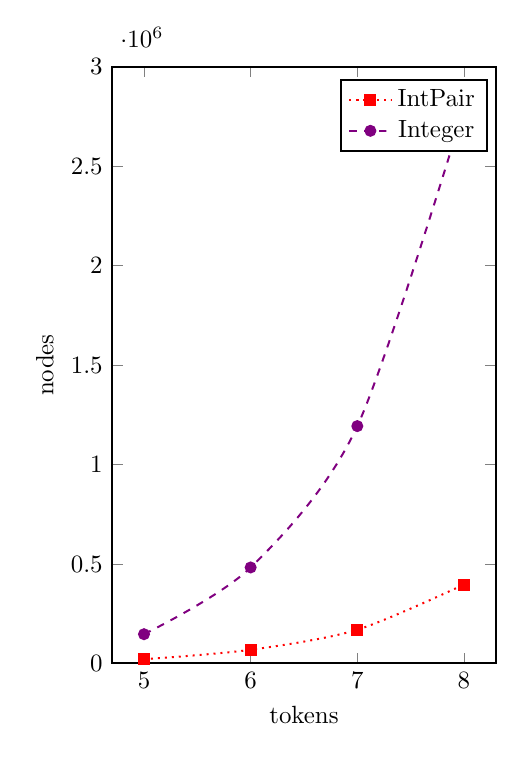
\begin{tikzpicture} [scale=0.9] 
	\begin{axis}[
	%  axis y line*=left,
	  ymin=0, ymax=3000000,
	  xlabel=tokens,
	  ylabel=nodes,
	  xtick=data]
		\addplot[smooth,mark=square*, mark options={solid},red, dotted]
		  coordinates{
		    (5,20879)
		    (6,68523)
		    (7,169435)
		    (8,396625)
		}; \label{pnt_plot} \addlegendentry{IntPair}
		\addplot[smooth,mark=*,mark options={solid},violet, dashed]
		  coordinates{
		    (5,146895)
		    (6,482543)
		    (7,1193363)
		    (8,2791621)
		}; \label{int_plot} \addlegendentry{Integer}
	\end{axis}
\end{tikzpicture}
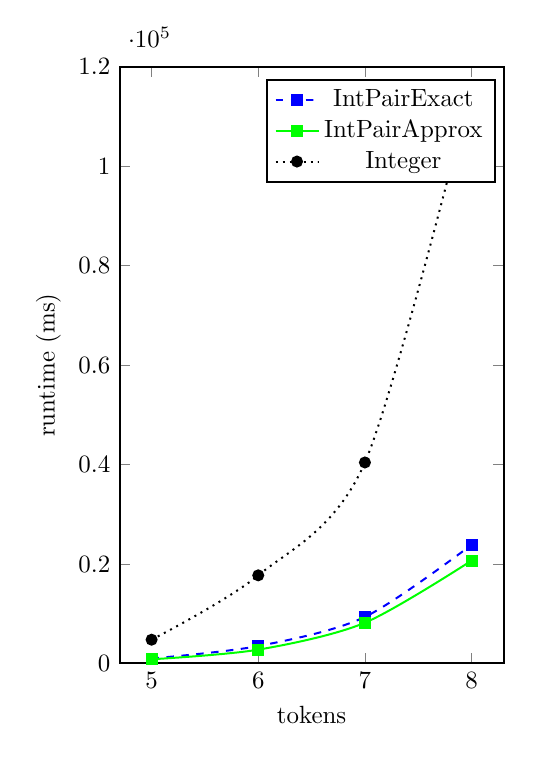
\begin{tikzpicture} [scale=0.9]
	
	\begin{axis}[
	%  boarders=all,
%	  axis y line*=right,
	%  axis x line=none,
	 xlabel=tokens,
	  ymin=0, ymax=120000,
	  xtick=data,
	  ylabel=runtime (ms) ] 
	  
	  
		\addplot[smooth,mark=square*,mark options={solid},blue, dashed]
		  coordinates{
		    (5,992)
		    (6,3491)
		    (7,9352)
		    (8,23866)
		}; \label{IntPairExact Run}
		
		\addplot[smooth,mark=square*,mark options={solid},green]
		  coordinates{
		    (5,827)
		    (6,2767)
		    (7,8186)
		    (8,20679)
		}; \label{IntPairApprox Run}
		
		\addplot[smooth,mark=*,mark options={solid},black, dotted]
		  coordinates{
		    (5,4770)
		    (6,17716)
		    (7,40416)
		    (8,116126)
		}; \label{IntegerRun}
	
		\addlegendentry{IntPairExact}
		\addlegendentry{IntPairApprox}
		\addlegendentry{Integer}
	\end{axis}
\end{tikzpicture}

\caption{{States=15, Maxcost=3, Steps=6}}
\end{figure}
%\begin{figure}[H]
%\begin{tikzpicture} [scale=1.8]
%	\pgfplotsset{
%	    scale only axis,
%		legend style={at={(0,0.8)}, anchor=west, font=\tiny},
%	    xmin=5, xmax=8
%	}
%	\begin{axis}[
%	  axis y line*=left,
%	  ymin=0, ymax=3000000,
%	  xlabel=tokens,
%	  ylabel=nodes,
%	  xtick=data]
%		\addplot[smooth,mark=square*, mark options={solid},red, dashdotted]
%		  coordinates{
%		    (5,20879)
%		    (6,68523)
%		    (7,169435)
%		    (8,396625)
%		}; \label{pnt_plot} \addlegendentry{IntPair Nodes}
%		\addplot[smooth,mark=square*,mark options={solid},violet, dashdotdotted]
%		  coordinates{
%		    (5,146895)
%		    (6,482543)
%		    (7,1193363)
%		    (8,2791621)
%		}; \label{int_plot} \addlegendentry{Integer Nodes}
%	\end{axis}
%	
%	\begin{axis}[
%	  axis y line*=right,
%	  axis x line=none,
%	  ymin=0, ymax=120000,
%	  ylabel=runtime (ms) ] 
%	  				\addlegendimage{/pgfplots/refstyle=pnt_plot}\addlegendentry{IntPair Nodes}
%	  				\addlegendimage{/pgfplots/refstyle=int_plot}\addlegendentry{Integer Nodes}
%	  
%	  
%		\addplot[smooth,mark=*,mark options={solid},blue, dashed]
%		  coordinates{
%		    (5,992)
%		    (6,3491)
%		    (7,9352)
%		    (8,23866)
%		}; \label{IntPairExact Run}
%		
%		\addplot[smooth,mark=*,mark options={solid},green]
%		  coordinates{
%		    (5,827)
%		    (6,2767)
%		    (7,8186)
%		    (8,20679)
%		}; \label{IntPairApprox Run}
%		
%		\addplot[smooth,mark=*,mark options={solid},black, dotted]
%		  coordinates{
%		    (5,4770)
%		    (6,17716)
%		    (7,40416)
%		    (8,116126)
%		}; \label{IntegerRun}
%	
%		\addlegendentry{IntPairExact Run}
%		\addlegendentry{IntPairApprox Run}
%		\addlegendentry{Integer Run}
%	\end{axis}
%\end{tikzpicture}
%\caption{{States=15, Maxcost=3, Steps=6}}
%\end{figure}

\begin{figure}[H]
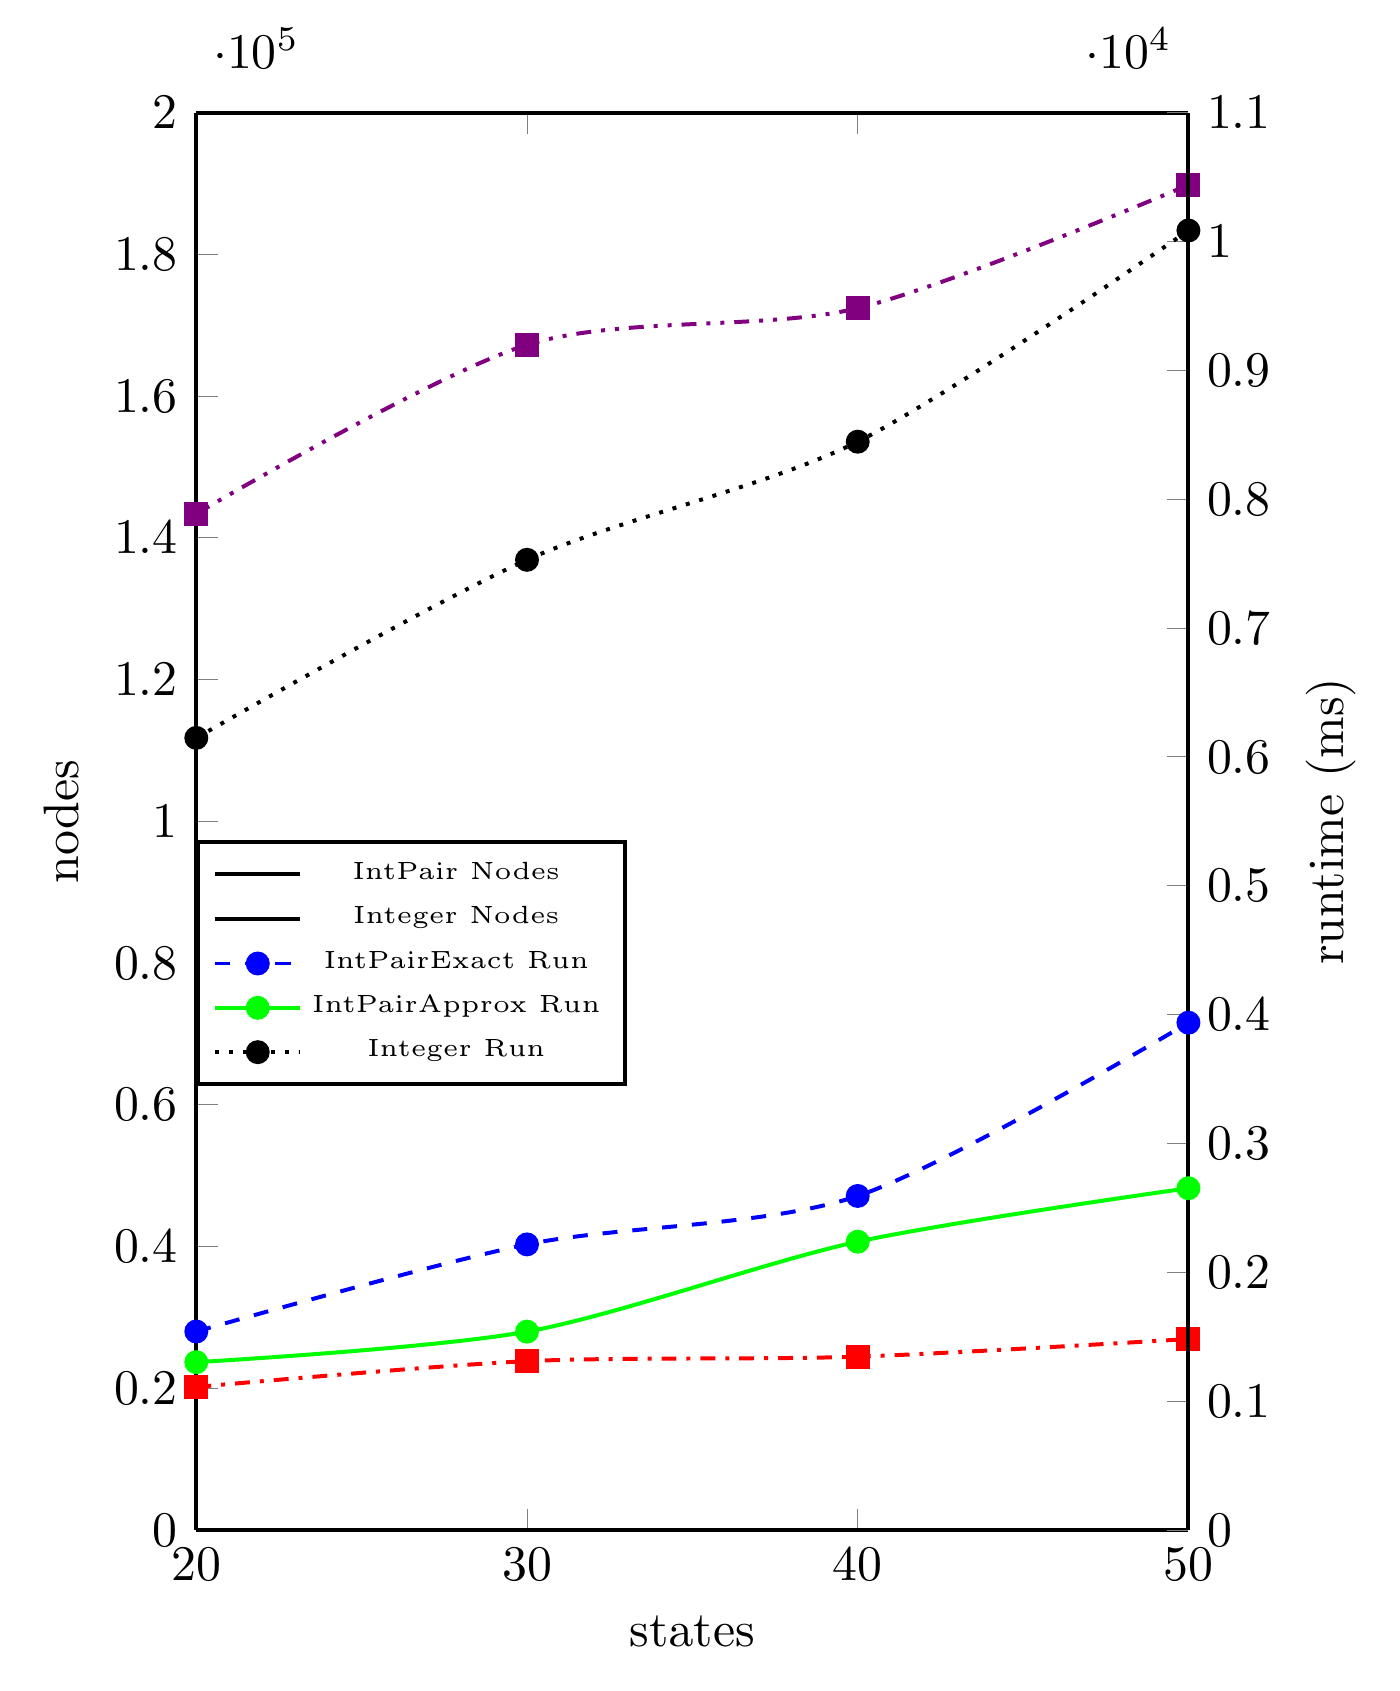
\begin{tikzpicture} [scale=1.8]
	\pgfplotsset{
	    scale only axis,
		legend style={at={(0,0.4)}, anchor=west, font=\tiny},
	    xmin=20, xmax=50
	}
	\begin{axis}[
	  axis y line*=left,
	  ymin=0, ymax=200000,
	  xlabel=states,
	  ylabel=nodes,	
	  xtick=data]
		\addplot[smooth,mark=square*,mark options={solid},red, dashdotted]
		  coordinates{
		  (20,20189)
		  (30,23833)
		  (40,24467)
		  (50,26959)
		}; \label{pns_plot} \addlegendentry{IntPair Nodes}
		\addplot[smooth,mark=square*,mark options={solid},violet, dashdotdotted]
		  coordinates{
		  (20,143413)
		  (30,167251)
		  (40,172417)
		  (50,189809)
		}; \label{ins_plot} \addlegendentry{Integer Nodes}
	\end{axis}
	
	\begin{axis}[
	  axis y line*=right,
	  axis x line=none,
	  ymin=0, ymax=11000,
	  ylabel=runtime (ms) ] 
	  				\addlegendimage{/pgfplots/refstyle=pns_plot}\addlegendentry{IntPair Nodes}
	  				\addlegendimage{/pgfplots/refstyle=ins_plot}\addlegendentry{Integer Nodes}
		\addplot[smooth,mark=*,mark options={solid},blue, dashed]
		  coordinates{
		  (20,1541)
		  (30,2217)
		  (40,2593)
		  (50,3938)
		}; \label{IntPairExact Run}
		
		\addplot[smooth,mark=*,mark options={solid},green]
		  coordinates{
		  (20,1303)
		  (30,1540)
		  (40,2238)
		  (50,2653)
		}; \label{IntPairApprox Run}
		
		\addplot[smooth,mark=*,mark options={solid},black, dotted]
		  coordinates{
		  (20,6148)
		  (30,7530)
		  (40,8447)
		  (50,10086)
		}; \label{IntegerRun}
	
		\addlegendentry{IntPairExact Run}
		\addlegendentry{IntPairApprox Run}
		\addlegendentry{Integer Run}
	\end{axis}
\end{tikzpicture}
\caption{{Token=5, Maxcost=3, Steps=6}}
\end{figure}

\begin{figure}[H]
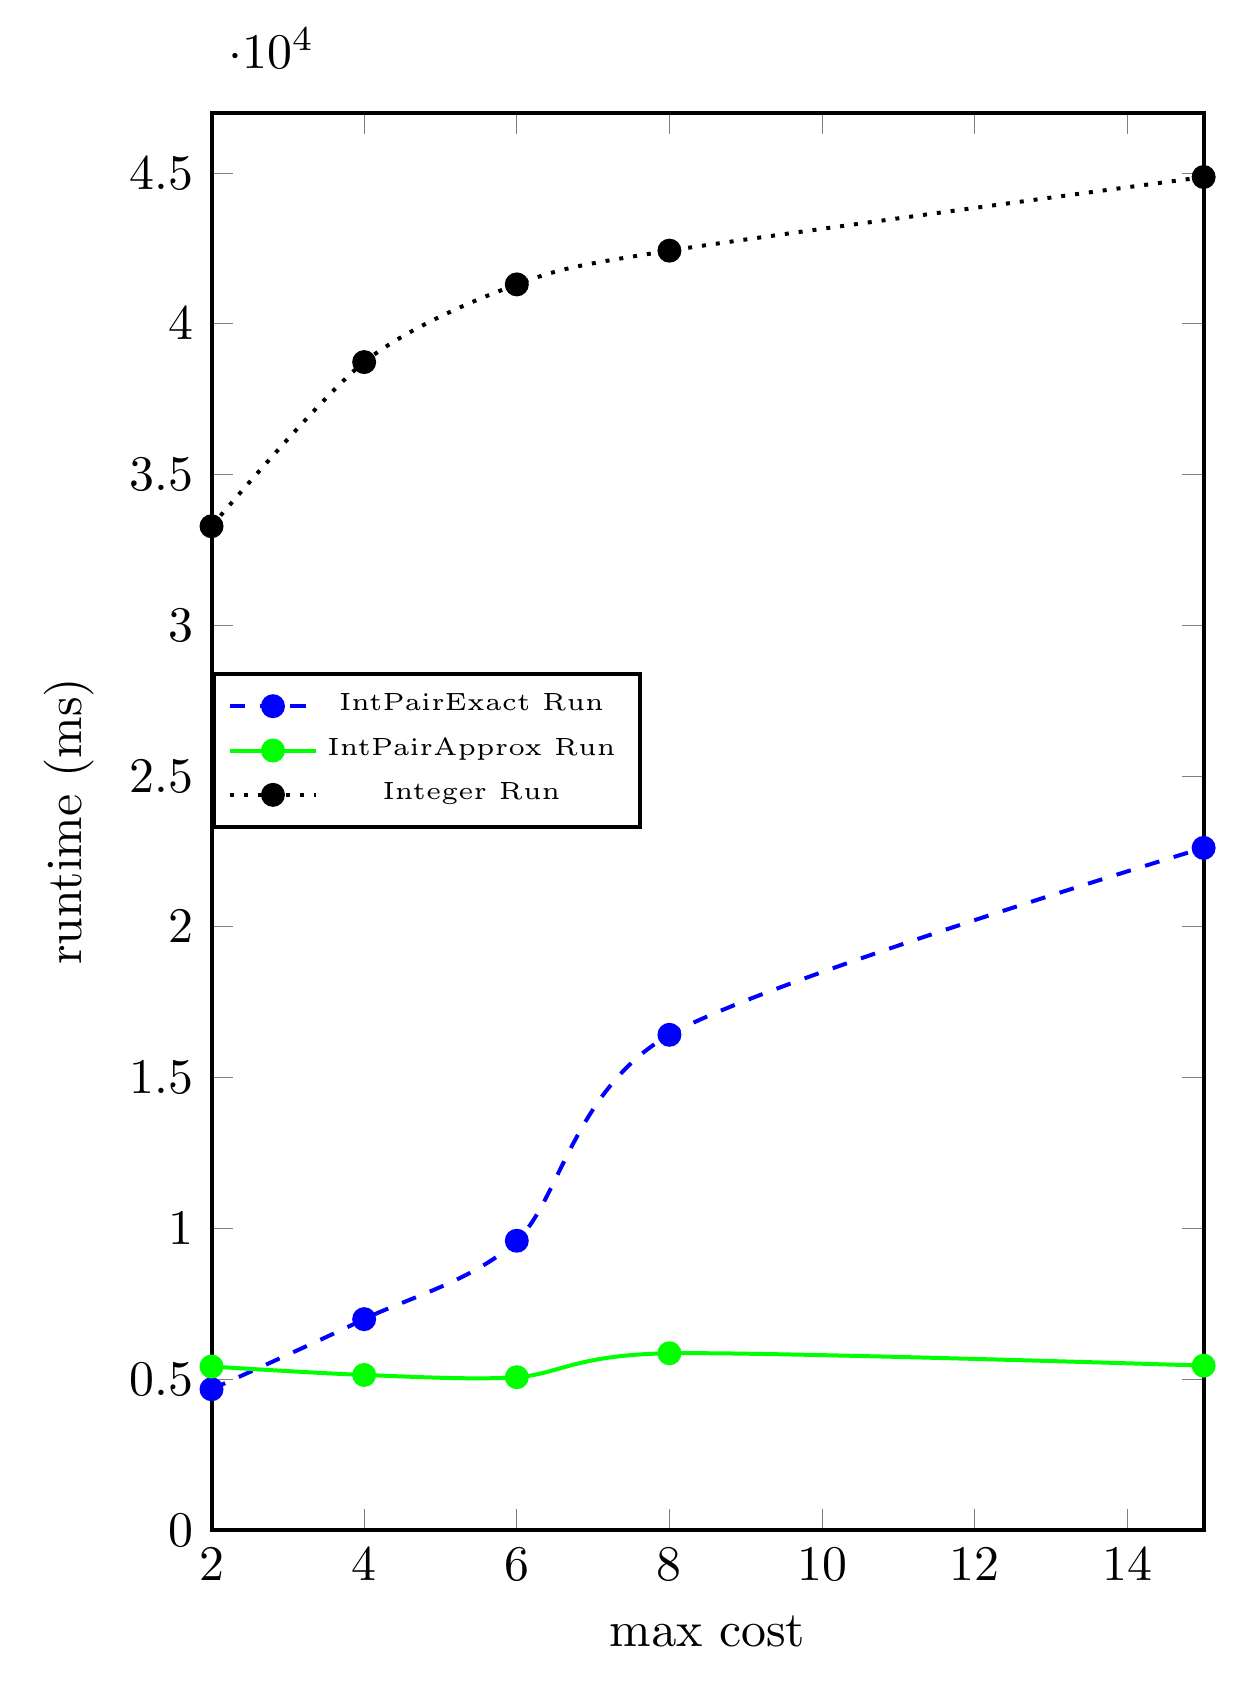
\begin{tikzpicture} [scale=1.8]
	\pgfplotsset{
	    scale only axis,
		legend style={at={(0,0.55)}, anchor=west, font=\tiny},
	    xmin=2, xmax=15,
	  xlabel=max cost
	}
%	\begin{axis}[
%	  axis y line*=left,
%	  ymin=0, ymax=800000,
%	  ylabel=nodes,	
%	  xtick=data]
%		\addplot[smooth,mark=x,red]
%		  coordinates{
%		  (2,93227)
%		  (4,93227)
%		  (6,93227)
%		  (8,93227)
%		  (15,93227)
%		}; \label{pn_plot} \addlegendentry{IntPair Nodes}
%		\addplot[smooth,mark=x,blue]
%		  coordinates{
%		  (2,755629)
%		  (4,755629)
%		  (6,755629)
%		  (8,755629)
%		  (15,755629)
%		}; \label{in_plot} \addlegendentry{Integer Nodes}
%	\end{axis}
	
	\begin{axis}[
%	  axis y line*=right,
%	  axis x line=none,
	  ymin=0, ymax=47000,
	  ylabel=runtime (ms) ] 
%	  				\addlegendimage{/pgfplots/refstyle=pn_plot}\addlegendentry{IntPair Nodes}
%	  				\addlegendimage{/pgfplots/refstyle=in_plot}\addlegendentry{Integer Nodes} 
		\addplot[smooth,mark=*,mark options={solid},blue, dashed]
		  coordinates{
		  (2,4669)
		  (4,6994)
		  (6,9594)
		  (8,16423)
		  (15,22621)
		}; \label{IntPairExact Run}
		
		\addplot[smooth,mark=*,mark options={solid},green]
		  coordinates{
		  (2,5423)
		  (4,5143)
		  (6,5069)
		  (8,5862)
		  (15,5452)
		}; \label{IntPairApprox Run}
		
		\addplot[smooth,mark=*,mark options={solid},black, dotted]
		  coordinates{
		  (2,33288)
		  (4,38731)
		  (6,41307)
		  (8,42426)
		  (15,44868)
		}; \label{IntegerRun}
	
		\addlegendentry{IntPairExact Run}
		\addlegendentry{IntPairApprox Run}
		\addlegendentry{Integer Run}
	\end{axis}
\end{tikzpicture}
\caption{{Steps=20, Tokens=5, Steps=7. Number of nodes is omitted because it is constant. The number of nodes for Pairs are 93000 and for Integer 760000.}}
\end{figure}

\begin{figure}[H]
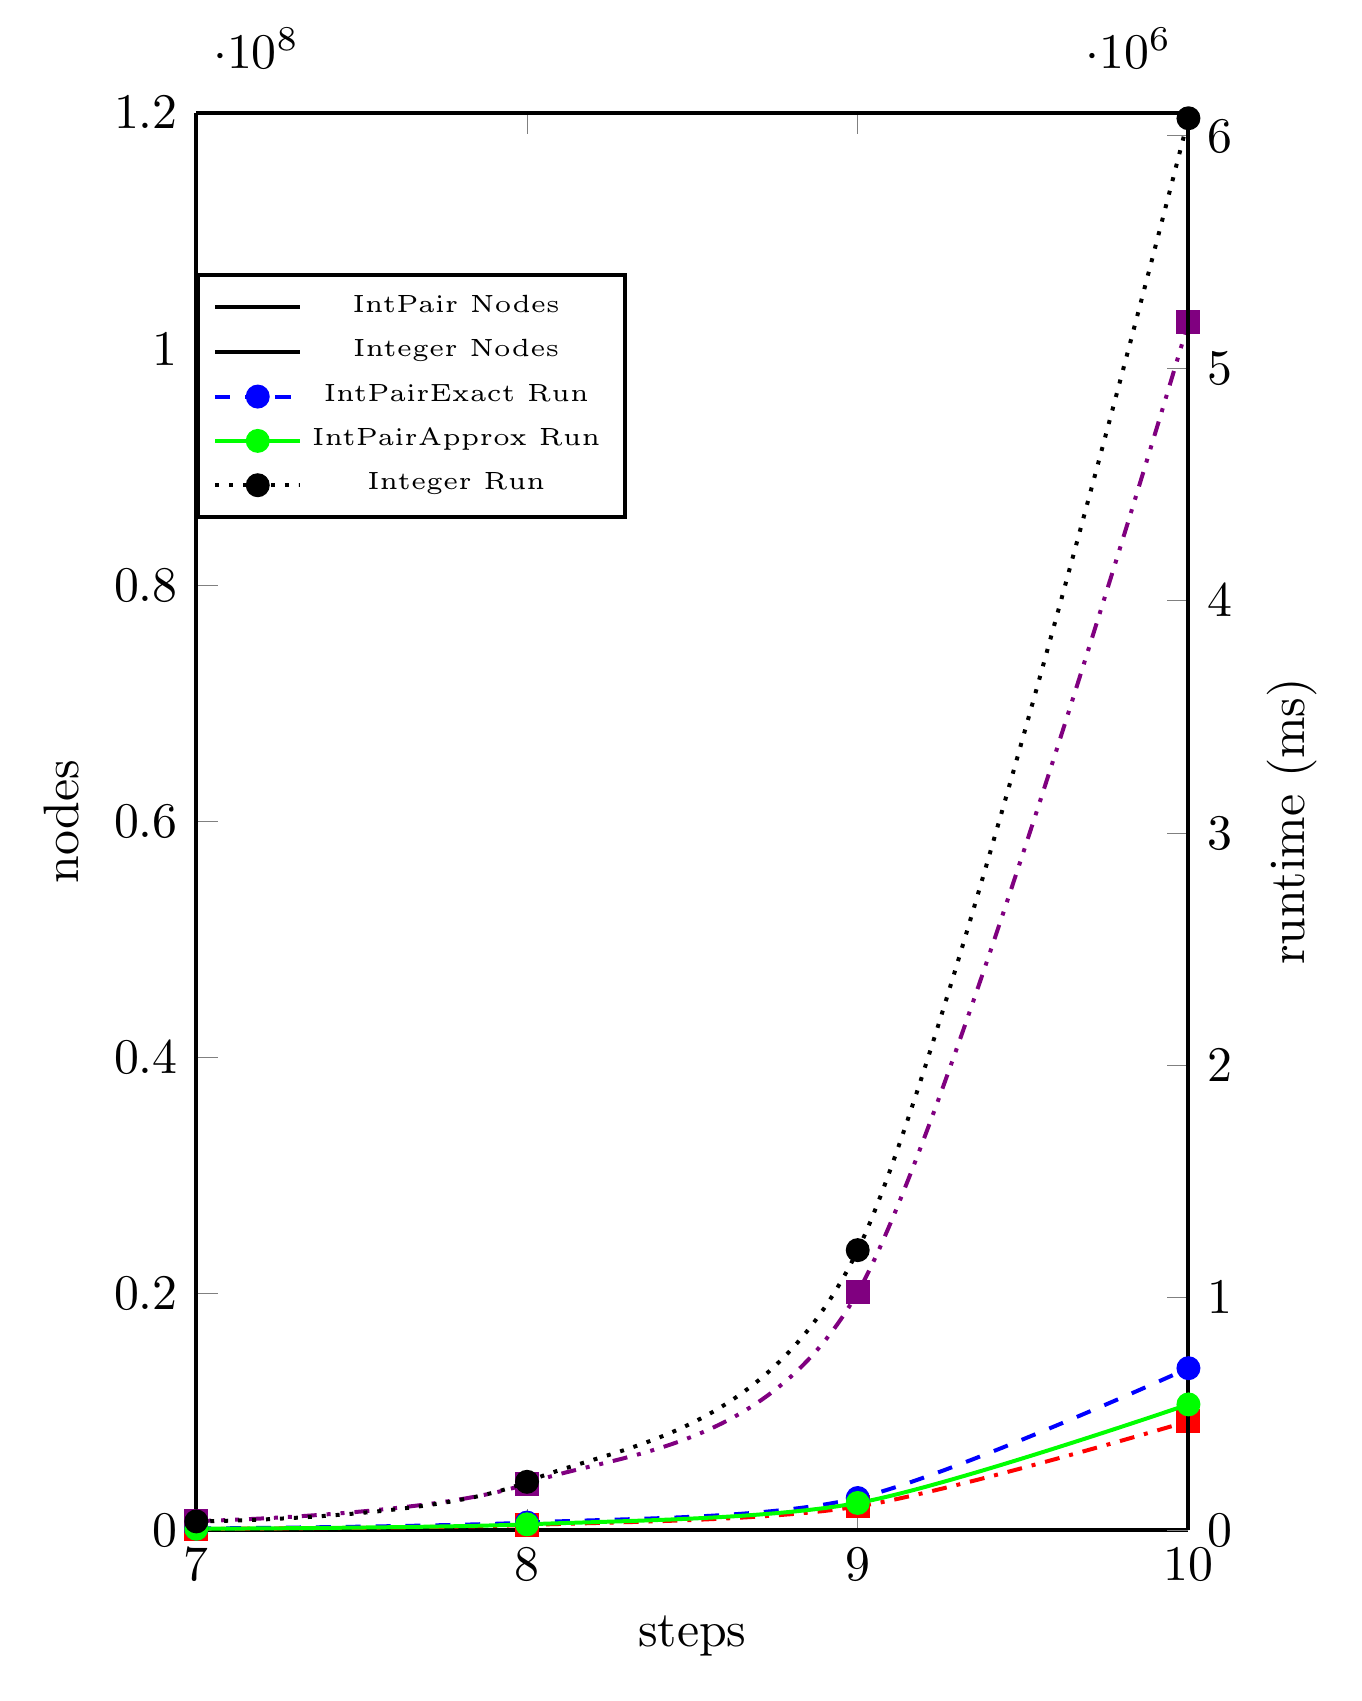
\begin{tikzpicture} [scale=1.8]
	\pgfplotsset{
	    scale only axis,
		legend style={at={(0,0.8)}, anchor=west, font=\tiny},
	    xmin=7, xmax=10
	}
	\begin{axis}[
	  axis y line*=left,
	  ymin=0, ymax=120000000,
	  xlabel=steps,
	  ylabel=nodes,	
	  xtick=data]
		\addplot[smooth,mark=square*,mark options={solid},red, dashdotted]
		  coordinates{
		  (7,93227)
		  (8,431051)
		  (9,1992011)
		  (10,9207489)
		}; \label{pnc_plot} \addlegendentry{IntPair Nodes}
		\addplot[smooth,mark=square*,mark options={solid},violet, dashdotdotted]
		  coordinates{
		  (7,755629)
		  (8,3924361)
		  (9,20128261)
		  (10,102243101)
		}; \label{inc_plot} \addlegendentry{Integer Nodes}
	\end{axis}
	
	\begin{axis}[
	  axis y line*=right,
	  axis x line=none,
	  ymin=0, ymax=6100000,
	  ylabel=runtime (ms) ] 
	  				\addlegendimage{/pgfplots/refstyle=pnc_plot}\addlegendentry{IntPair Nodes}
	  				\addlegendimage{/pgfplots/refstyle=inc_plot}\addlegendentry{Integer Nodes}
		\addplot[smooth,mark=*,mark options={solid},blue, dashed]
		  coordinates{
		  (7,6535)
		  (8,32150)
		  (9,137846)
		  (10,696655)
		}; \label{IntPairExact Run}
		
		\addplot[smooth,mark=*,mark options={solid},green]
		  coordinates{
		  (7,5582)
		  (8,24569)
		  (9,116613)
		  (10,540708)
		}; \label{IntPairApprox Run}
		
		\addplot[smooth,mark=*,mark options={solid},black, dotted]
		  coordinates{
		  (7,37169)
		  (8,207591)
		  (9,1204695)
		  (10,6076224)
		}; \label{IntegerRun}
	
		\addlegendentry{IntPairExact Run}
		\addlegendentry{IntPairApprox Run}
		\addlegendentry{Integer Run}
	\end{axis}
\end{tikzpicture}
\caption{{States=20, Tokens=5, Maxcost=4}}
\end{figure}

In the graphs we can see advantages for IntPair. In all tests they win over the regular integer solution in both execution time and the size of the search tree. However, it does so at the cost of higher memory usage per node. A node in the integer variant uses five integer variables, while the pair variant uses two pairs and one integer. The size of a node for the integer case should be roughly proportional to $Steps(States + Maxtotalcost)$ plus some overhead, but for the pair case the domain sizes of the pairs is proportional to the number of states times the max total cost. This means that the size per node is $Steps*States*Maxtotalcost$. For two-dimensional tuples with "normal" domain sizes this should not be of any concern. However, higher dimensions could cause trouble. The DFA problem could be modeled with a five-dimensional tuple. For the case in figure 2 with 50 states, 5 tokens, 6 steps and max total cost 18 the size per node would be around 100MB. Note though that the tuples have a higher memory usage \textit{per node} and that this does not necessarily mean that the total memory usage is higher since the number of nodes shrinks. The case where this would be a problem is if the search tree became to deep, because a parent node can not be freed from memory until its children have been propagated to either a failure or a solution.

For all situations the number of nodes are exactly equal for both IntPairExact and IntPairApprox. This may be a bit surprising. It would be reasonable that the number of nodes were, if ever so slightly, higher for IntPairApprox, since the domain is approximated. The reason is that if the starting state $s_0$ and the starting cumalative cost $c_0$ is assigned (which they are for a DFA), then everything else follows automatically if we branch on the tokens first. This is easy to see because $s_1=S(s_0, t_0)$ and $c_1=c_0+C(s_0, t_0)$. This is also confirmed by the fact that there were no failures during the execution. If we removed some values from the domains of $t_1$, $s_1$ and $c_1$ and above things would have been different. 

In figure 3 IntPairApprox seems to be almost constant in time. Even though this may seem very good it is not something that shows that tuples work, since the same result probably would be achievable by using an approximate version of integer variables for the cost. In the same graph we can read in the comment that the number of nodes were constant for all three methods. This is because how the DFA:s are generated. The random generator first generates the state matrix and then the cost matrix, so the automatons looks exactly the same except for the transition costs.

All in all the graphs indicates that tuples can give significantly better performance for certain problems. The only possible source of error with this experiment is that the reference propagator may not be optimized enough, but I find that highly unlikely. After all, the implementation of IntVar has to be assumed to be very optimized, and the reference propagator is much more optimized than the ones for pairs.

\section{Related Work}
The paper Propagating Regular Counting Constraints (Beldiceanu, Flener, Pearson, Van Hentenryck) describes constraints for a counter-DFA (cDFA). It is defined as a regular DFA with only accepting states and such that the transition function not only returns the next state, but the increase for a counter. The DFA in this thesis is almost identical. The main difference is that we also use non-accepting states. The other difference is more philosophical. Instead of counting we talk about cost, but it makes no difference in practise. I wanted to do a performance comparasion with that implementaion, but it would be complicated to do that in a fair way, because the constraints are implemented in Prolog, while everything in this thesis is in C++.

In Implementation of bit-vector variables in a CP solver (Dye) Gecode is used, and a new variable is implemented. That paper was useful for getting more understanding of how to implement a new variable in Gecode.

The paper A propagator design framework for constraints over sequences (Monette, Flener, Pearson) shows that tuples can be used to make pruning much more efficient. This thesis is basically a practical demonstration that this indeed is true, and that it translates directly into better performance.

\section{Conclusions and future work}
The tests shows that tuples have potential. Both of them perform better than the integer variant in both number of nodes and total execution time, and there is still much room for further improvement. Especially the vector operations are very inefficient and can easily be improved.

All big software libraries have coding standards. There is plenty of work to rewrite the code for IntPairs in such a way that it satisfies Gecodes standards. For instance, vector from std is not allowed. Furthermore, the code is far from ready in other aspects. It contains only the methods needed to run the tests in this thesis, that is, proving that tuples actually is a good idea. One example of this is that it exists methods to get the minimum and maximum x-value for the domain, but no methods for y-value. Also, the propagators and the brancher currently only accepts arrays. The brancher for IntPairApprox has a bug, which manifested itself by making the program producing the same solution several times which should not be possible. This does not matter in this thesis since it is not used.

In this thesis there is one exact and one approximate version. The approximation is exact in one dimension and only stores the boundaries for the second. This is just one way of doing it and there are several other ways of approximating the domain. Another relevant change that could be made is to extend the pairs to arbitrary dimensions.

\end{document}
